\documentclass{standalone}
\usepackage{tikz}

\begin{document}

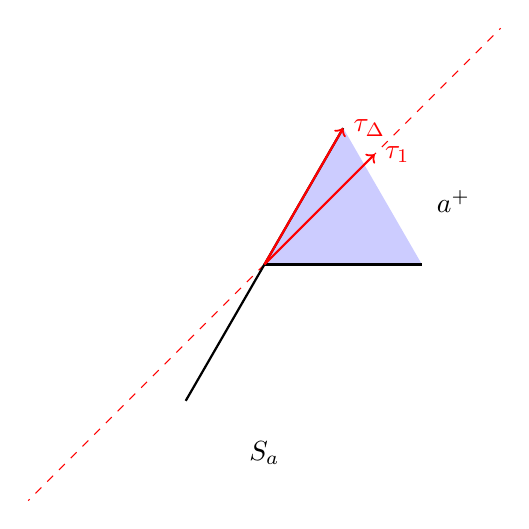
\begin{tikzpicture}[scale=2]
    % Draw the triangle
    \fill[blue!20] (0,0) -- (1,0) -- (0.5,0.866) -- cycle;
    
    % Draw the dashed lines
    \draw[dashed, red] (0,0) -- (1.5,1.5);
    \draw[dashed, red] (0,0) -- (-1.5,-1.5);
    
    % Draw the solid lines
    \draw[thick, black] (0,0) -- (1,0);
    \draw[thick, black] (0,0) -- (0.5,0.866);
    \draw[thick, black] (0,0) -- (-0.5,-0.866);
    
    % Label the vectors
    \draw[->, red, thick] (0,0) -- (0.7,0.7) node[right] {$\tau_{1}$};
    \draw[->, red, thick] (0,0) -- (0.5,0.866) node[right] {$\tau_{\Delta}$};
    
    % Label the region
    \node at (1.2,0.4) {$a^{+}$};
    \node at (0,-1.2) {$S_{a}$};
\end{tikzpicture}

\end{document}